\documentclass[12pt,a4paper]{scrartcl}
\usepackage[utf8]{inputenc}
\usepackage[T1]{fontenc}
\usepackage[french]{babel}
\usepackage{textcomp}
\usepackage{lmodern}
\usepackage{graphicx}
\usepackage[dvipsnames,svgnames]{xcolor}
\usepackage{microtype}
\usepackage{listings}
\usepackage{hyperref} \hypersetup{colorlinks=true,linkcolor=Brown,urlcolor=Navy,
breaklinks=true,pdfstartview=XYZ}
\usepackage{fancyhdr} 
\title{Rapport projet I62}
\author{Tom Bartier, Nino Cantera, Balbony Ivano}

\begin{document}
\pagestyle{fancy}
\fancyhead{} % clear all header fields
\fancyhead[RO,LE]{\textbf{Compte Rendu TP I62}}

\maketitle


\begin{abstract}
Ce rapport concerne le projet du module I62 Génie Logiciel de la L3 Informatique
de l'université de Toulon. Le but de ce projet était de nous faire découvrir
les différents concepts théoriques du génie logiciel et de les appliquer sur un projet 
pratique travaillé pendant les séances de TP ainsi qu'en dehors des heures de cours.
\end{abstract}

\tableofcontents

\section {Introduction}

Notre projet était de mettre au point un simulateur de rover explorant la planète Mars.
L'application est en mode client / serveur, elle permet à l'utilisateur de contrôler un rover
et d'explorer la planète Mars avec d'autres utilisateurs, d'analyser différents matériaux
ou encore de déployer un drone afin de faciliter l'exploration.

\subsection{Infos Pratiques}
L'application ne peut se lancer que si le serveur est allumé. 
Pour lancer le serveur, executez la commande \lstinline!python ./src/server/app-server.py <ip> <port>!
où <ip> correspond à l'adresse ip de votre machine et <port> désigne le port sur lequel le
serveur attendra les connexions. Exemple : \lstinline!python ./src/server/app-server.py 127.0.0.1 25025! \\\\
Pour lancer l'application client, executez la commande python ./src/client/app-client.py <ip> <port>

Côté client vous arrivez sur la page de connexion, deux comptes sont disponibles :
\begin{enumerate}
    \item Utilisateur : bob     Mot de Passe : 1234
    \item Utilisateur : alice   Mot de Passe : 5678
\end{enumerate}

\section{Exigences}
Voici les exigences mises en place pour ce projet, à noter qu'elles n'ont pas toutes pu être implémentées
mais qu'elles pourraient l'être si le projet venait à être continué après ce rendu.

\subsection{Interactions client/serveur}

\begin{itemize}

\item EX\_SERV\_0002
\begin{itemize}
\item S'authentifier
\item Le SI doit permettre à l'utilisateur de s'authentifier grâce à un
		identifiant et un mot de passe.
\end{itemize}


\item EX\_SERV\_0003
\begin{itemize}
\item Voir les autres
\item Le SI doit permettre à l'utilisateur de voir les autres autres 
	utilisateur dans l'environement
\end{itemize}

\item EX\_SERV\_0004
\begin{itemize}
\item Stockage environement
\item Le SI héberge sur le serveur l'environement dans lequel évoluent les 
	rovers.
\end{itemize}


\end{itemize}

\subsection{GUI}

\begin{itemize}

\item EX\_GUI\_0001
\begin{itemize}
\item Avancer
\item Le SI doit permettre à l'utilisateur de faire avancer le rover.
\end{itemize}

\item EX\_GUI\_0002
\begin{itemize}
\item Reculer
\item Le SI doit permettre à l'utilisateur de faire reculer le rover.
\end{itemize}

\item EX\_GUI\_0003
\begin{itemize}
\item Pivoter
\item Le SI doit permettre à l'utilisateur de faire pivoter le rover dans les 			deux sens (sens horaire et antihoraire).
\end{itemize}

\item EX\_GUI\_0004
\begin{itemize}
\item Contrôler la vitesse
\item Le SI doit permettre à l'utilisateur de contrôler la vitesse du rover.
\end{itemize}

\item EX\_GUI\_005
\begin{itemize}
\item Utiliser Laser
\item Le SI doit permettre à l'utilisateur de tirer un laser sur un rocher.
\end{itemize}


\item EX\_GUI\_0006
\begin{itemize}
\item Surveiller énergie
\item Le SI doit permettre à l'utilisateur de surveiller la quantité d'énergie
		restante au rover.
\end{itemize}

\item EX\_GUI\_0007
\begin{itemize}
\item Analyser
\item Le SI doit permettre à l'utilisateur d'obtenir les informations sur la 
		matière pulvérisée et analysée par le rover.
\end{itemize}

\item EX\_GUI\_0008
\begin{itemize}
\item Creuser
\item Le SI doit permettre à l'utilisateur d'indiquer au rover de creuser dans
		le sol à l'aide de sa foreuse
\end{itemize}

\item EX\_GUI\_0009
\begin{itemize}
\item Pilote Automatique
\item Le SI doit permettre à l'utilisateur de mettre le rover en mode pilote 
		automatique.
\end{itemize}		

\item EX\_GUI\_00010
\begin{itemize}
\item Mode Manuel
\item Le SI doit permettre à l'utilisateur de mettre le rover en mode manuel.
\end{itemize}
		
\item EX\_GUI\_0011
\begin{itemize}
\item Allumer
\item Le SI doit permettre à l'utilisateur d'allumer le rover.
\end{itemize}

\item EX\_GUI\_0012
\begin{itemize}
\item Eteindre
\item Le SI doit permettre à l'utilisateur d'éteindre le rover.
\end{itemize}

\item EX\_GUI\_0013
\begin{itemize}
\item Mini carte
\item Le SI doit permettre à l'utilisateur de consulter une mini carte de la planète (en ne voyant clairement que les zones découvertes).
\end{itemize}

\item EX\_GUI\_0014
\begin{itemize}
\item Affichage température
\item Le SI doit permettre à l'utilisateur de consulter la température actuelle 
		de la zone.
\end{itemize}

\end{itemize}

\subsection{Caméra}

\begin{itemize}


\item EX\_CAM\_0001
\begin{itemize}
\item Affichage Caméra
\item Le SI doit permettre à l'utilisateur de voir le retour de la caméra en 
		temps réel.
\end{itemize}

\item EX\_CAM\_0002
\begin{itemize}
\item Pivoter Caméra
\item Le SI doit permettre à l'utilisateur de faire pivoter la caméra dans 
	tous les sens.
\end{itemize}

\item EX\_CAM\_0003
\begin{itemize}
\item Zoom
\item Le SI doit permettre à l'utilisateur de zoomer et dézoomer la caméra. 
\end{itemize}


\item EX\_CAM\_0004
\begin{itemize}
\item Prendre des photos
\item Le SI doit permettre à l'utilisateur de prendre des photos avec la caméra 			et de les enregistrer sur sa machine.
\end{itemize}

\item EX\_CAM\_0005
\begin{itemize}
\item Prendre des vidéos
\item Le SI doit permettre à l'utilisateur de prendre des vidéos.
\end{itemize}

\item EX\_CAM\_0006
\begin{itemize}
\item Pivoter
\item Le SI doit permettre à l'utilisateur de faire pivoter la caméra.
\end{itemize}

\item EX\_CAM\_0007
\begin{itemize}
\item Enregistrer Photos
\item Le SI doit permettre à l'utilisateur d'enregistrer les photos prises.
\end{itemize}

\item EX\_CAM\_0008
\begin{itemize}
\item Enregistrer Photos
\item Le SI doit permettre à l'utilisateur d'enregistrer les vidéos prises.
\end{itemize}

\end{itemize}

\subsection{Rover}

\begin{itemize}

\item EX\_ROVER\_0001
\begin{itemize}
\item S'abîmer
\item Le SI doit infliger des dégâts au rover en cas de colision avec un obstacle ou en cas de chute.
\end{itemize}

\item EX\_ROVER\_0002
\begin{itemize}
\item Panne d'énergie
\item Le SI doit permettre au rover de tomber en panne d'énergie.
\end{itemize}

\item EX\_ROVER\_0003
\begin{itemize}
\item Recharge d'énergie
\item Le SI doit permettre au rover de se recharger en énergie.
\end{itemize}

\item EX\_ROVER\_0004
\begin{itemize}
\item Remplacer foreuse
\item Le SI doit permettre au rover d'abandonner sa foreuse et la remplacer par 
		une autre si la première se retrouve coincée ou endommagée.
\end{itemize}

\item EX\_ROVER\_0005
\begin{itemize}
\item Découvrir les alentours
\item Le SI doit permettre au rover de découvrir les alentours.
\end{itemize}

\item EX\_ROVER\_0006
\begin{itemize}
\item Prévoir météo
\item Le SI doit permettre au rover de prévoir de prévoir le prochain évènement
		météorologique de la zone où il se trouve.
\end{itemize}

\end{itemize}

\subsection {Hélicoptère}

\begin{itemize}

\item EX\_HELI\_0001
\begin{itemize}
\item Déployer hélicopter
\item Le SI doit permettre au rover de déployer l'hélicoptère
\end{itemize}

\item EX\_HELI\_0002
\begin{itemize}
\item Ranger hélicopter
\item Le SI doit permettre au rover de ranger l'hélicoptère
\end{itemize}

\item EX\_HELI\_0003
\begin{itemize}
\item Monter
\item Le SI doit permettre à l'utilisateur de faire monter l'hélicoptère
\end{itemize}

\item EX\_HELI\_0004
\begin{itemize}
\item Descendre
\item Le SI doit permettre à l'utilisateur de faire descendre l'hélicoptère
\end{itemize}

\item EX\_HELI\_0005
\begin{itemize}
\item Avancer
\item Le SI doit permettre à l'utilisateur de faire avancer l'hélicoptère
\end{itemize}

\item EX\_HELI\_0006
\begin{itemize}
\item Reculer
\item Le SI doit permettre à l'utilisateur de faire reculer l'hélicoptère
\end{itemize}

\item EX\_HELI\_0007
\begin{itemize}
\item Aller à gauche
\item Le SI doit permettre à l'utilisateur de faire aller l'hélicoptère vers la gauche
\end{itemize}

\item EX\_HELI\_0008
\begin{itemize}
\item Aller à droite
\item Le SI doit permettre à l'utilisateur de faire aller l'hélicoptère vers la droite
\end{itemize}

\item EX\_HELI\_0009
\begin{itemize}
\item Pivoter
\item Le SI doit permettre à l'utilisateur de faire pivoter l'hélicoptère
\end{itemize}

\item EX\_HELI\_0010
\begin{itemize}
\item Caméra Hélico
\item Le SI doit permettre à l'utilisateur contrôler la caméra de l'hélicoptère (voir rubrique Caméra)
\end{itemize}

\item EX\_HELI\_0011
\begin{itemize}
\item Energie
\item Le SI doit permettre à l'hécoptère de pouvoir tomber en panne d'énergie
\end{itemize}

\item EX\_HELI\_0012
\begin{itemize}
\item Energie
\item L'hécoptère doit pouvoir recharger son énergie en se posant rentrant à terre.
\end{itemize}

\item EX\_HELI\_0013
\begin{itemize}
\item Décollage
\item Le SI doit permettre à l'hélicoptère de décoller
\end{itemize}

\item EX\_HELI\_0014
\begin{itemize}
\item Aterrissage
\item Le SI doit permettre à l'hélicoptère d'atterrir
\end{itemize}

\item EX\_HELI\_0015
\begin{itemize}
\item Vitesse
\item Le SI doit permettre à l'utilisateur de changer la vitesse de l'hélicoptère
\end{itemize}

\item EX\_HELI\_0016
\begin{itemize}
\item Décollage
\item Le SI doit permettre à l'utilisateur de mettre l'hélicoptère en mode automatique.
\end{itemize}

\item EX\_HELI\_0016
\begin{itemize}
\item Cartographier
\item Le SI doit permettre à l'hélicoptère de cartographier ses environs
\end{itemize}

\end{itemize}

\subsection{Environnement}

\begin{itemize}

\item EX\_ENV\_0001
\begin{itemize}
\item Brouillard
\item Le SI affiche à l'utilisateur un brouillard dans les zones non découvertes par le rover et l'hélicoptère
\end{itemize}

\item EX\_ENV\_0002
\begin{itemize}
\item Rocher
\item Le SI dispose des rochers dans l'environement
\end{itemize}

\item EX\_ENV\_0002
\begin{itemize}
\item Rocher
\item Le SI dispose de différents niveaux de hauteur dans l'environement
\end{itemize}

\item EX\_ENV\_0003
\begin{itemize}
\item Tempête de poussière
\item Le SI dispose d'un évènement "tempête de poussière" sur une zone qui
		réduit la distance de vision et endommage un petit peu l'hélicoptère 
		lorsqu'il est en vol et empêche la recharge d'énergie solaire.
\end{itemize}

\item EX\_ENV\_0004
\begin{itemize}
\item Vent
\item Le SI dispose d'un évènement "vent" sur une zone avec différents niveaux d'intensité qui vont avoir une influence sur l'hélicoptère.
\end{itemize}

\end{itemize}

\section {Diagrammes}
Voici les différents diagrammes UML réalisés pour le projet, séparés en deux catégories, d'abord les diagrammes 
du serveur puis ceux du client.

\subsection{Diagrammes Serveur}
\begin{figure}[h]
    \centering
    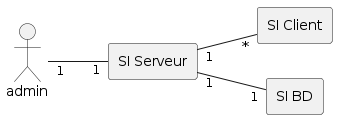
\includegraphics[width=0.5\textwidth]{DiagCS_Admin.png}
    \caption{Diagramme de Contexte Statique Serveur}\label{cs_serv}
\end{figure}

\begin{figure}[h]
    \centering
    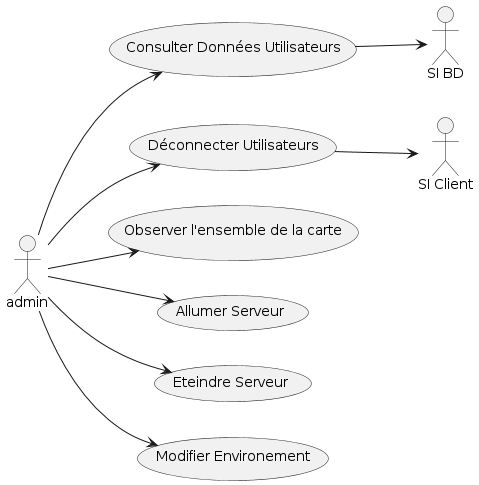
\includegraphics[width=0.5\textwidth]{Diag_Seq_Admin.png}
    \caption{Diagramme de Séquence Serveur}\label{cs_serv}
\end{figure}

\end{document}